%%%%%%%%%%%%%%%%%%%%%%%%%%%%%%%%%%%%%%%%%
% Short Sectioned Assignment
% LaTeX Template
% Version 1.0 (5/5/12)
%
% This template has been downloaded from:
% http://www.LaTeXTemplates.com
%
% Original author:
% Frits Wenneker (http://www.howtotex.com)
%
% License:
% CC BY-NC-SA 3.0 (http://creativecommons.org/licenses/by-nc-sa/3.0/)
%
%%%%%%%%%%%%%%%%%%%%%%%%%%%%%%%%%%%%%%%%%

%----------------------------------------------------------------------------------------
%	PACKAGES AND OTHER DOCUMENT CONFIGURATIONS
%----------------------------------------------------------------------------------------

\documentclass[paper=a4, fontsize=11pt]{scrartcl} % A4 paper and 11pt font size

\usepackage[T1]{fontenc} % Use 8-bit encoding that has 256 glyphs
%\usepackage{fourier} % Use the Adobe Utopia font for the document - comment this line to return to the LaTeX default
\usepackage[english]{babel} % English language/hyphenation
\usepackage{amsmath,amsfonts,amsthm} % Math packages
\usepackage{bm}
\usepackage{lipsum} % Used for inserting dummy 'Lorem ipsum' text into the template
\usepackage{graphicx} % This one is for pictures
\usepackage{sectsty} % Allows customizing section commands
\allsectionsfont{\centering \normalfont\scshape} % Make all sections centered, the default font and small caps
\usepackage{color}
\usepackage{float}
\floatplacement{figure}{H}
\usepackage{fancyhdr} % Custom headers and footers
\pagestyle{fancyplain} % Makes all pages in the document conform to the custom headers and footers
\fancyhead{} % No page header - if you want one, create it in the same way as the footers below
\fancyfoot[L]{} % Empty left footer
\fancyfoot[C]{} % Empty center footer
\fancyfoot[R]{\thepage} % Page numbering for right footer
\renewcommand{\headrulewidth}{0pt} % Remove header underlines
\renewcommand{\footrulewidth}{0pt} % Remove footer underlines
\setlength{\headheight}{13.6pt} % Customize the height of the header

%\numberwithin{equation}{section} % Number equations within sections (i.e. 1.1, 1.2, 2.1, 2.2 instead of 1, 2, 3, 4)
%\numberwithin{figure}{section} % Number figures within sections (i.e. 1.1, 1.2, 2.1, 2.2 instead of 1, 2, 3, 4)
%\numberwithin{table}{section} % Number tables within sections (i.e. 1.1, 1.2, 2.1, 2.2 instead of 1, 2, 3, 4)

%\setlength\parindent{0pt} % Removes all indentation from paragraphs - comment this line for an assignment with lots of text

%----------------------------------------------------------------------------------------
%	TITLE SECTION
%----------------------------------------------------------------------------------------

\newcommand{\horrule}[1]{\rule{\linewidth}{#1}} % Create horizontal rule command with 1 argument of height

\title{	
\normalfont \normalsize 
\textsc{Columbia University -- Fall 2013} \\ [25pt] % Your university, school and/or department name(s)
\horrule{0.5pt} \\[0.4cm] % Thin top horizontal rule
\huge Machine Learning Homework \#4\\ % The assignment title
\horrule{2pt} \\[0.5cm] % Thick bottom horizontal rule
}

\author{Joe Ellis - jge2105} % Your name

\date{\normalsize\today} % Today's date or a custom date

\begin{document}

\maketitle % Print the title

%----------------------------------------------------------------------------------------
%	PROBLEM 1
%----------------------------------------------------------------------------------------

\section{Problem 1 -- EM Derivation}
In this problem we will derive the Expectation-Maximization algorithm for a mixture of multinomials.
Suppose, that $x$ is represented as a vector such that $x(j) = 1$ if $x$ takes the $j^{th}$ value, and $\sum_j x(j) = 1$.
The distribution of $x$ is described by a mixture of $K$ discrete multinomials such that:

\begin{align}
p(x) = \sum_{k=1}^K \pi_k p(x|\mu_k)
\end{align}

where 

\begin{align}
p(x|\mu_k) = \prod_{j=1}^M \mu_k(j)^{x(j)}.
\end{align}

Where $\pi_k$ is the mixing coefficients, and $\mu_k$ specifies the parameters of the $k^th$ component.
We then must derive the Expectation and Maximization steps to maximize the log-likelihood of an observed data set $\{x_i\}$.

\subsection{Expectation Step}
First we want to calculate what is referred to in EM as the responsibilities of each data point given the mixtures.
To do this we want to find the $p(z_i|x_i;\theta)$, where $z_i$ is the mixture that this data point belongs to.
In this way, we can estimate the likelikhood that each data point was generated by one of the given mixtures, and then weight our estimates in the maximization step accordingly.

\begin{align}
p(z_i|x_i|;\theta) &= \frac{p(x_i|z_i;\theta)p(z_i)}{p(xi)},	\ by Bayes Rule \\
&= \frac{p(x_i|z_i;\theta)\pi_k}{p(xi)} \\
&= \frac{p(x_i|\mu_k)\pi_k}{\sum_{k=1}^K \pi_k p(x|\mu_k)} \\
&= \frac{\pi_k\mu_k^{x_i(j)}}{\sum_{k=1}^K \pi_k\mu_k^{x_i(j)})}. \\
\end{align}

Therefore, we have the responsibilities of each data point, and have calculated how likely each data point was generated from each mixture.

\subsection{Maximization Step}
Now that we have the responsibilities we will in turn now calculate the parameters $\mu_k$ and $\pi_k$ that maximize the log-likelihood function of the seen data.
Let's find the log-likelihood of the data given our hidden variables $\theta$, to do this, we must maximize the general form of the equation below.

\begin{align}
\theta := \underset{\theta}{\operatorname{argmax}}\sum_{i=1}^N \sum_{z_i}(Q_i(z_i)\frac{p(x_i,z_i;\theta)}{Q_i(z_i)}).
\end{align}

In the above equation $Q_i(z_i)$ is the value for each mixture and data point that is calculated using the E-step from above.
In the derivation below we will use the notation $\tau_{k,i}$, where $\tau_{k,i} = Q_i(z_k)$.
Let's refer to the above equation as $l(\theta)$

\begin{align}
l(\theta) &= \sum_{i=1}^N \sum_{k=1}^K \tau_{k,i} log(\frac{p(x_i,z_i;\theta)}{\tau_{k,i}} \\
&= \sum_{i=1}^N \sum_{k=1}^K \tau_{k,i} log(p(x_i,z_i;\theta)) -  \sum_{i=1}^N \sum_{k=1}^K \tau_{k,i} log( \tau_{k,i}) \\
&= \sum_{i=1}^N \sum_{k=1}^K \tau_{k,i} log(p(x_i,z_i;\theta)) -  const \\
&=  \sum_{i=1}^N \sum_{k=1}^K \tau_{k,i} log( \pi_k\prod_{j=1}^M \mu_k(j)^{x_i(j)}) \\
&= \sum_{i=1}^N \sum_{k=1}^K \tau_{k,i} log(\pi_k) + \sum_{j=1}^M log(\mu_k(j)^{x_i(j)}) \\
&= \sum_{i=1}^N \sum_{k=1}^K \tau_{k,i} log(\pi_k) + \tau_{k,i}\sum_{j=1}^M x_i(j) log(\mu_k(j)) \\.
\end{align}

Now that we have derived the log likelihood we must maximize the above equation with respect to the parameters $\mu$ and $\pi$.
However the derivation is not straight forward and we must use laplaclian variables to satisfy the constraints of, $\sum_j \mu_k(j) = 1$ and $\sum_k \pi_k = 1$.

Therefore, let's do the derivation.
We set the derivative with respect to $\mu_k(j)$ and the constraints with laplace variable $\lambda$ to zero and solve.

\begin{align}
\frac{\partial l(\theta)}{\partial \mu_k(j)} &=\frac{\partial}{\partial \mu_k(j)}  \sum_{i=1}^N \sum_{k=1}^K \tau_{k,i} log(\pi_k) + \tau_{k,i}\sum_{j=1}^M x_i(j) log(\mu_k(j)) - \sum_{k=1}^K \lambda_k (\sum_{j=1}^M \mu_k(j) -1) \\
&=  \sum_{i=1}^N  \tau_{k,i} \frac{1}{\mu_k(j)} - \lambda_k = 0. \\
\end{align}

Thus, 

\begin{align}
\mu_k(j) =  \frac{\sum_{i=1}^N x_i(j) \tau_{k,i}}{\lambda_k}.
\end{align}

Plugging $\mu_k(j)$ back into the equation, $\sum_{j=1}^M \mu_k(j) -1)$ gives us the equation for $\lambda_k$ below,

\begin{align}
\lambda_k = \sum_{i=1}^N \sum_{m=1}^M \tau_{k,i} x_i(m).
\end{align}

So therefore we have the update for our $\mu_k(j)$ as, 

\begin{align}
\mu_k(j) = \frac{\sum_{i=1}^N \tau_{k,i} x_i(j)}{\sum_{i=1}^N \sum_{m=1}^M \tau_{k,i} x_i(m)}
\end{align}

Similarly, we can derive the value for the other parameter $\pi_k$, with laplacian constraints.

\begin{align}
\frac{\partial l(\theta)}{\partial \pi_k} &=\frac{\partial}{\partial \pi_k}  \sum_{i=1}^N \sum_{k=1}^K \tau_{k,i} log(\pi_k) + \tau_{k,i}\sum_{j=1}^M x_i(j) log(\mu_k(j)) - \lambda (\sum_{k=1}^K \pi_k -1) \\
&=  \sum_{i=1}^N  \tau_{k,i} \frac{1}{\pi_k} - \lambda = 0. \\
\end{align}

Thus, 

\begin{align}
\pi_k =  \frac{\sum_{i=1}^N \tau_{k,i}}{\lambda}.
\end{align} 

Plugging $\lambda$, back into the constraint equation, $\sum_{k=1}^K \pi_k -1)$, we solve for lambda, 

\begin{align}
\lambda &= \sum_{i=1}^N \sum_{k=1}^K \tau_{k,i} \\
& = N.
\end{align}

So, therefore we have the update for our mixing coefficients ($\pi_k$) as,

\begin{align}
\pi_k = \frac{\sum_{i=1}^N \tau_{k,i}}{N} \\
\end{align}

Therefore, we have derived the entire EM algorithm for a mixture of multinomials.


%----------------------------------------------------------------------------------------
%	PROBLEM 2
%----------------------------------------------------------------------------------------
\section{Problem 2}

\subsection{Mixtures of Gaussians}
Using the code provided to us in the tutorial section of the class website we were able to perform EM on a mixture of gaussians on two datasets.
The figures generated from the EM algorithm and the gaussian distributions found are superimposed over the data points.

Figures \ref{fig:datasetA} and \ref{fig:datasetB} show the results of the EM calculation.

\begin{figure}
\centering
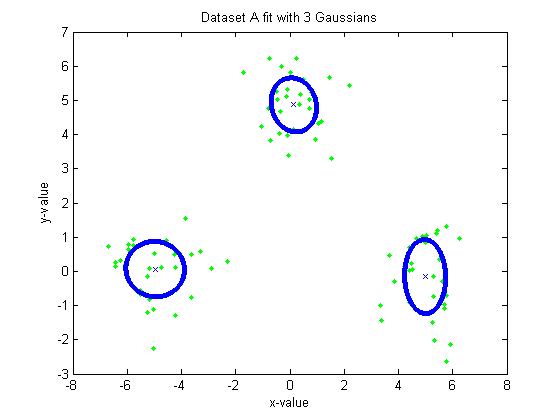
\includegraphics[width=0.5\textwidth]{datasetA.png}
\caption{EM result on dataset A using 3 Gaussian distributions}
\label{fig:datasetA}
\end{figure}

\begin{figure}
\centering
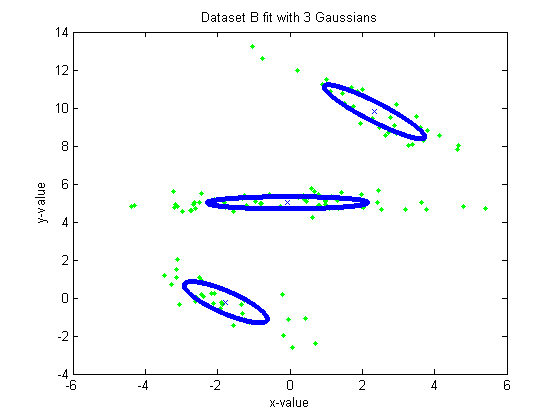
\includegraphics[width=0.5\textwidth]{datasetB.png}
\caption{EM result on dataset B using 3 Gaussian distributions}
\label{fig:datasetB}
\end{figure}

\subsection{Mixtures of Multinomials}
In this section we explore using the derivation provided in section 1 to create a mixture of multinomials model to differentiate between plays written by Shakespeare and Middleton.
We have 9 plays written by Shakespeare and 9 plays written by Middleton, and we will try to classify how we well we can separate the two using multiple mixture models.

% Test Results for the Matlab functions
% K = 1
%The average training log-likelihood is
%mean_train_logs =
 % -3.0650e+06
%The training standard deviation is
%std_train_logs =
%   2.7029e+04
%The average testing log-likelihood is
%mean_test_logs =
 % -8.7940e+05
%The testing standard deviation is
%std_testing_logs =
%  2.7718e+04
% K = 2
%The average training log-likelihood is
%mean_train_logs =
% -3.0927e+06
%The training standard deviation is
%std_train_logs =
%   2.4745e+04
%The average testing log-likelihood is
%mean_test_logs =
%  -8.8021e+05
%The testing standard deviation is
%std_testing_logs =
%   2.4963e+04
% K = 3
%The average training log-likelihood is
%mean_train_logs =
% -3.0906e+06
%The training standard deviation is
%std_train_logs =
%   1.9562e+04
%The average testing log-likelihood is
%mean_test_logs =
%  -8.9373e+05
%The testing standard deviation is
%std_testing_logs =
%   1.9783e+04
% K = 4
%The average training log-likelihood is
%mean_train_logs =
%  -3.1112e+06
%The training standard deviation is
%std_train_logs =
%   3.5735e+04
%The average testing log-likelihood is
%mean_test_logs =
%  -8.8161e+05
%The testing standard deviation is
%std_testing_logs =
%   3.6037e+04
%the trainign log-likelihoods

We began by implementing the EM algorithm with multinomial counts for documents clustering and classification.  
The results were very promising, and the responsibilities for each document after the EM algorithm were correctly classified into Shakespeare and Middleton.
We can see below the mixture for each document moving to the correct responsibilities for some given random initialization with 2 assumed mixtures.  
To see how the responsibilities change throughout the EM algorithm, I have shown the responsibilities for each document after 1 iteration, 5 iterations, and convergence (36 iterations).
These results can be seen in Figures \ref{fig:randinit}, \ref{fig:iter}, and \ref{fig:classificationacc}.
As we can see from the graphs below the results converge to the proper responsibilities for each document, and we receive 100\% accuracy.

\begin{figure}
\centering
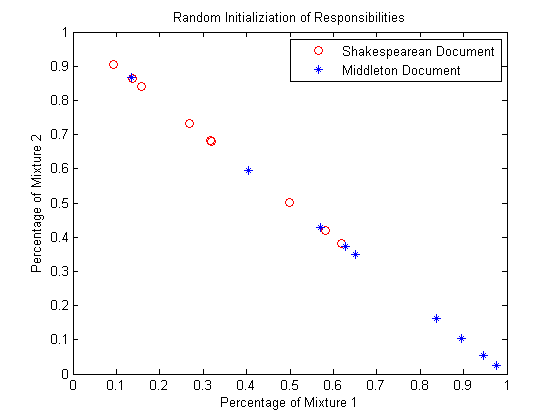
\includegraphics[width=0.3\textwidth]{RandInit.png}
\caption{Document responsibilities after 1 iteration}
\label{fig:randinit}
\end{figure}

\begin{figure}
\centering
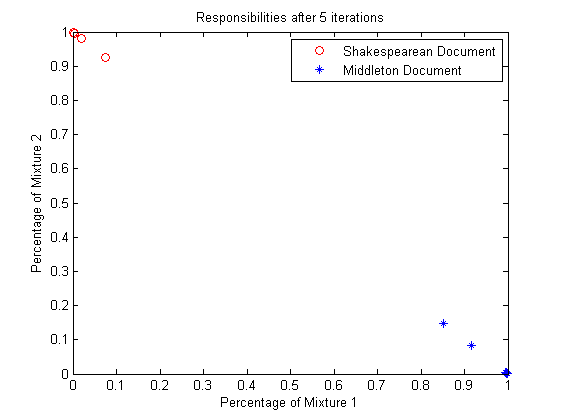
\includegraphics[width=0.3\textwidth]{5iter.png}
\caption{Document responsibilities after 5 iterations}
\label{fig:iter}
\end{figure}

\begin{figure}[H]
\centering
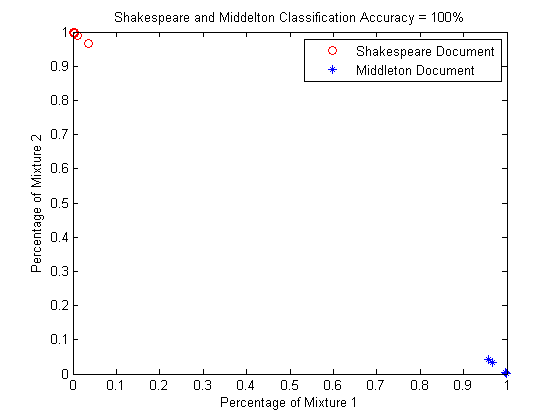
\includegraphics[width=0.3\textwidth]{classification_acc.png}
\caption{Final document responsibilities}
\label{fig:classificationacc}
\end{figure}

We can also see how the log-likelihood evolves during the EM algorithm.
This is shown in Figure \ref{fig:ll}.

\begin{figure}
\centering
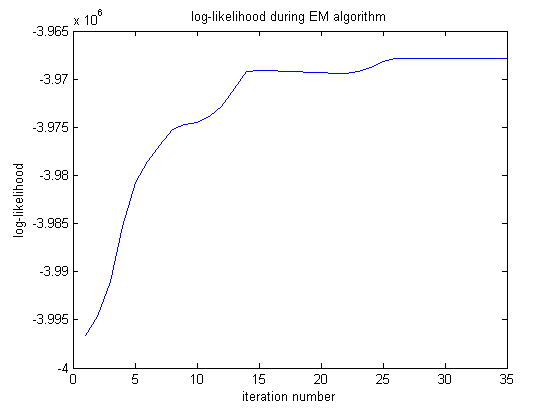
\includegraphics[width=0.5\textwidth]{log-likelihood.png}
\caption{Log-likelihood during the EM algorithm}
\label{fig:ll}
\end{figure}

Finally, we want to decide the amount of mixtures that we should use on this type of data.
To do this we removed 2 of the documents at random from each author in the training set, and then determined the log-likelihood of those models given our learned model on the rest of the data.
The values for the average log-likelihood of the train and test set and standard deviation of the log-likelihood for train and test can be seen in Table \ref{tab:mm}.
We can see that as the number of mixtures used $K$ rises we have overfitting on the training set and lowering log-likelihood. 
 However, for most of the examples on the training sets we have larger K improves the log-likelihood which makes sense.
It appears that using 2 or 1 mixture makes the most sense for this result, which makes some logical sense because there are 2 authors, but they may not have a large difference in writing style.

\begin{table}
\centering
\label{tab:mm}
\caption{Log-Likelihood results for different numbers of multinomial mixtures}
\begin{tabular}{|c|c|c|c|c|}
\hline
Mixture Number ($K$) & ave train $l(\theta)$ & std train $l(\theta)$  & ave test $l(\theta)$  &  std test $l(\theta)$  \\ \hline \hline
K=1 & -3.0650e+06 & 2.7029e+04 &  -8.7940e+05 & 2.7718e+04 \\ \hline
K=2 &  -3.0927e+06 & 2.4745e+04 & -8.8021e+05 &  2.4963e+04 \\ \hline
K=3 & -3.0906e+06 & 1.9562e+04 & -8.9373e+05 & 1.9783e+04 \\ \hline
K=4 & -3.1112e+06 & 3.5735e+04 & -8.8161e+05 & 3.6037e+04 \\ \hline
\end{tabular}
\end{table}


The only issue that I had creating this program was that the responsibilities were converging on 1 and 0 to quickly, and causing problems.  
Therefore, to slow down the convergence and allow for the EM algorithm to work I divided the document probabilities for each mixture by 1000, and this solved the issue.  
Instead of the log probabilities for the documents being possibly 1000 values apart, they were then only 1 to 2 integers apart allowing for proper conversion.  
This fix can be seen in line 81 of ``mix\_mult\_model.m''.



%----------------------------------------------------------------------------------------
%	PROBLEM 3
%----------------------------------------------------------------------------------------
\section{Problem 3}

\subsection{Part A}
In this section we will prove that the arithmetic mean on non-negative numbers is at least their geometric mean.
First let's define the arithmetic mean and geometric mean for some set of numbers.  
Assume we have the set $X$, where $X = \{x_1,x_2,...,x_N\} $ and $ x_i \in \mathbb{P}^+$.
The arithmetic mean can be found as follows, 

\begin{align}
mean_{arithmetic} = \frac{\sum_i x_i}{N}.
\end{align}

The geometric mean can be found as follows,

\begin{align}
mean_{geometric} = \sqrt[N]{\prod_i x_i}
\end{align}

We will use Jensen's Inequality with natural logarithm to prove that the arithmetic mean is always larger than the geometric mean.

\begin{align}
log(mean_{arithmetic}) &= log(\frac{\sum_i xi}{N}) \\
&= log(\frac{x_1}{N}+\frac{x_2}{N}+...+\frac{x_N}{N}) \\
&\ge \frac{1}{N}log(x_1)+\frac{1}{N}log(x_2)+...+\frac{1}{N}log(x_N), \ by \  Jensen \\
&= log(\sqrt[N]{x_1}\sqrt[N]{x_2}...\sqrt[N]{x_N}) \\
&=log(\sqrt[N]{x_1x_2...x_N}) \\
&= log(mean_{geometric})
\end{align}

Since we know that $log$ is a strictly increasing function, then we have proven that $ mean_{arithmetic} > mean_{geometric}$.

\subsection{Part B}
Now we want to prove using Jensen's inequality that, 

\begin{align}
\sum_i exp(\theta^Tf_i) &\ge exp( \theta^T \sum_i \alpha_if_i - \sum_i \alpha_i log(\alpha_i)), \\
&where\   \alpha_i = \frac{ exp(\theta^Tf_i)}{\sum_j  exp(\theta^Tf_i)}.
\end{align}

First we notice that the set of constant variables $\sum_i \alpha_i = 1$, and are therefore they are weights on each point.
Using this knowledge, we can then use Jensen's inequality on this problem.
We also know that the function $exp$, is convex and therefore using Jensen's Inequality we know, $\sum_i \alpha_i exp(x_i) \ge exp(\sum_i \alpha_i x_i)$.
Let's start with the right side of the equation, and simplify it.
Thus, 

\begin{align}
 \theta^T \sum_i \alpha_if_i - \sum_i \alpha_i log(\alpha_i) &=  \theta^T \sum_i \alpha_if_i - \sum_i \alpha_i log(\frac{exp(\theta^Tf_i)}{\sum_j exp(\theta^Tf_j)}) \\
&=  \theta^T \sum_i \alpha_if_i - \sum_i \alpha_i (log(exp(\theta^Tf_i)) - log(\sum_j exp(\theta^Tf_j))) \\
&= \theta^T \sum_i \alpha_if_i - (\sum_i \alpha_i \theta^T f_i -  \sum_i  \alpha_i  log(\sum_j exp(\theta^Tf_j))) \\
&=  \theta^T \sum_i \alpha_if_i - \sum_i \alpha_i \theta^T f_i + \sum_i  \alpha_i  log(\sum_j exp(\theta^Tf_j)) \\
&=  \theta^T \sum_i \alpha_if_i - \theta^T \sum_i \alpha_i f_i + \sum_i  \alpha_i  log(\sum_j exp(\theta^Tf_j)) \\
& =  \sum_i  \alpha_i  log(\sum_j exp(\theta^Tf_j)) \\
& \le  log( \sum_i \alpha_i \sum_j exp(\theta^T f_j)) \\
&= log( \sum_i \frac{exp(\theta^T f_i)}{\sum_j exp(\theta^Tf_j)}\sum_j exp(\theta^Tf_j)) \\
&= log(\sum_i exp(\theta^T f_i)). \\
\end{align}

Now if we plug this upper bound, because $exp$ is strictly increasing, into our original inequality we get, 

\begin{align}
 exp( \theta^T \sum_i \alpha_if_i - \sum_i \alpha_i log(\alpha_i)) &\le exp( log(\sum_i exp(\theta^T f_i))) \\
&= \sum_i exp(\theta^T f_i).
\end{align}

Therefore, we have shown what we wanted to prove.
\end{document}